\section{The \fedhep{} Methodology}
\label{sec:method}
\label{sec:overview}

\paragraph{High-Level Workflow}
Figure~\ref{fig:architecture} and Algorithm~\ref{alg:fedhep} summarize the overall architecture and execution workflow of \fedhep{}. On-device, each client maintains a single shared convolutional backbone $\Phi_\theta$ feeding three linear heads ($W_r, W_p, W_l$), applying Active-Class Logit Masking (ACLM) and skew-calibrated loss weighting to suppress absent-class interference. For peer discovery, clients compress updates into random sketches $\mathbf{s}_i$. On the server, Root updates and backbones are aggregated via Subspace-Constrained Cosine Filtering (SCCF), adaptive norm clipping, and Temporal Trust Tracking (TTT).


\paragraph{Problem Formulation}
We consider a distributed federated network of $N$ heterogeneous edge clients $\mathcal{N} = \{1, \dots, N\}$. Each client $i$ possesses a private local training dataset $\mathcal{D}_i = \{(x_j, y_j)\}_{j=1}^{n_i}$ sampled from distribution $\mathcal{P}_i(x, y)$ over input space $\mathcal{X}$ and label space $\mathcal{Y} = \{0, 1, \dots, C-1\}$. We denote the subset of classes present on client $i$ by $\mathcal{Y}_i = \{y \in \mathcal{Y} \mid \exists (x, y) \in \mathcal{D}_i\}$. Under non-IID Dirichlet label partitioning, edge clients typically observe only a fraction of the total classes ($|\mathcal{Y}_i| \ll C$).

\paragraph{Threat Model}
We consider a Byzantine adversary controlling up to a fraction $q < 0.5$ of clients $\mathcal{M} \subset \mathcal{N}$ executing coordinated attacks~\cite{fang2020local,bhagoji2019analyzing,shejwalkar2021manipulating}:
(1) \textit{Label Flipping}: malicious nodes map training labels symmetrically via $y \to C - 1 - y$;
(2) \textit{Sign Flipping}: updates are inverted and scaled via $\Delta \mathbf{w} \to -\gamma \Delta \mathbf{w}$ (with scaling factor $\gamma > 0$);
(3) \textit{Gradient Ascent}: implemented as an amplified update reversal $\Delta \mathbf{w} \to -5\,\Delta \mathbf{w}$ (versus $\gamma=1.5$ for Sign Flipping), which pushes the aggregate to ascend the training loss; and
(4) \textit{Gaussian Noise}: updates are replaced with random Gaussian vectors $\mathcal{N}_{\mathrm{Gauss}}(0, \sigma^2 \mathbf{I})$.
The central server maintains no clean proxy validation dataset and cannot inspect private client data.

\subsection{Hierarchical Representation Architecture}
\label{sec:architecture}

\paragraph{Architecture Overview and Intuition}
Personalized federated learning on edge devices faces a fundamental tension between model expressiveness and on-device resource constraints. Conventional dual-model formulations (e.g., Ditto~\cite{li2021ditto}) maintain two full neural network instances per client---one global consensus model and one personalized model---which roughly doubles parameter storage, backpropagation activations, and peak VRAM. Conversely, decoupled-head approaches (e.g., FedRep~\cite{collins2021exploiting}) train a single backbone alongside an isolated local head, but omit peer collaboration; when local training data is scarce under severe label skew, these isolated heads are prone to overfitting on narrow class subsets. \fedhep{} addresses this trade-off by introducing a tripartite classifier hierarchy built on top of a single shared convolutional feature extractor $\Phi_\theta: \mathcal{X} \to \mathbb{R}^d$. Rather than duplicating backbones or isolating clients, \fedhep{} structures classification capacity into three complementary tiers: (1)~a globally aggregated Root head ($W_r$) capturing invariant representations common across all $N$ clients; (2)~a collaborative Parent head ($W_p$) synchronized among peer clients within cluster $\mathcal{C}_k$ sharing overlapping label distributions; and (3)~a private Local head ($W_l$) optimized on-device without communication. During on-device training, Active-Class Logit Masking (ACLM) shields the shared backbone from gradient interference caused by unobserved classes, while skew-calibrated loss weighting dynamically shifts capacity across tiers based on empirical label entropy. During inference, predictions are formed through a temperature-calibrated linear ensemble of the three heads, achieving strong personalization accuracy and tail fairness within the footprint of a single edge model.

\paragraph{Three-Tier Classifier Heads on a Single Backbone}
Specifically, each client maintains a single convolutional feature extractor $\Phi_\theta: \mathcal{X} \to \mathbb{R}^d$ parameterized by weights $\theta$, where $d$ denotes the feature representation dimension (e.g., $d = 512$). Branched directly from the terminal feature representation $\Phi_\theta(x)$ are three linear classification heads $W_h \in \mathbb{R}^{d \times C}$ indexed by tier $h \in \{r, p, l\}$, where $C$ is the total class count: the Root head $W_r$ (aggregated globally across $\mathcal{N}$ via Byzantine-resilient consensus), the Parent head $W_p$ (synchronized within peer cluster $\mathcal{C}_{k(i)}$), and the Local head $W_l$ (trained locally on-device).

During on-device inference, predictions are computed by an anchored linear combination of temperature-calibrated logits~\cite{guo2017calibration}:
\begin{equation}
\label{eq:ensemble}
\mathbf{z}_{\mathrm{ens}} = w_l \frac{\mathbf{z}_i^{(l)}}{T_l} + w_p \frac{\mathbf{z}_i^{(p)}}{T_p} + w_r \frac{\mathbf{z}_i^{(r)}}{T_r}, \quad \hat{y} = \argmax_{c \in \mathcal{Y}} z_{\mathrm{ens}, c},
\end{equation}
where $\mathbf{z}_i^{(h)} = W_h^\top \Phi_\theta(x) \in \mathbb{R}^C$ is the logit vector produced by tier $h \in \{r, p, l\}$, $z_{\mathrm{ens}, c}$ denotes the $c$-th coordinate of composite logit $\mathbf{z}_{\mathrm{ens}}$, $\hat{y} \in \mathcal{Y}$ is the predicted class label, and $T_h > 0$ are fixed head-specific temperature scalars that calibrate prediction confidence across heads (empirically set to $T_r = 1.0$, $T_p = 0.8$, and $T_l = 0.5$). The coefficients $w_h \ge 0$ (satisfying $\sum_{h} w_h = 1$) denote inference ensemble weights, which are initialized from the skew-calibrated training weights $\alpha_h$ derived below and refined online. At evaluation, \fedhep{} restricts the argmax to the client's observed classes $\mathcal{Y}_i$ (closed-set inference) in the main benchmarks; baselines in those benchmarks use unrestricted argmax (see the open-set results in Section~\ref{sec:exp_results}).

\begin{figure*}[t]
    \centering
    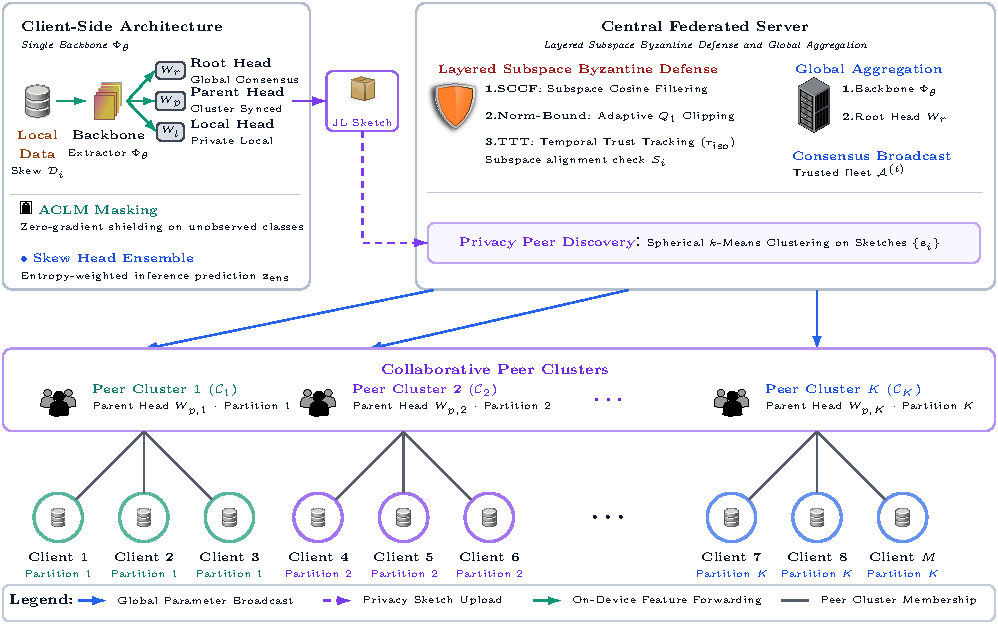
\includegraphics[width=0.82\textwidth]{figures/fedhep_hierarchy_figure.pdf}
    \caption{Overview of FedHEP Architecture. (Left) On-device client with a single backbone, tripartite head ensemble. (Right) Server-side sketch clustering and layered subspace defense.}
    \label{fig:architecture}
\end{figure*}

\paragraph{Active-Class Logit Masking (ACLM)}
In standard cross-entropy training, computing the softmax denominator over all $C$ classes forces the network to assign non-zero probabilities to unobserved classes. When a client only possesses a subset of classes $\mathcal{Y}_i \subset \mathcal{Y}$, evaluating standard cross-entropy penalizes these missing categories, driving their logits toward $-\infty$ and injecting destructive negative gradient updates that degrade the shared backbone $\Phi_\theta$~\cite{menon2021long}.

To mitigate this gradient interference, \fedhep{} applies Active-Class Logit Masking (\textbf{ACLM}) to the Parent and Local heads. For client $i$ with observed class set $\mathcal{Y}_i$, the masked logit coordinate for class $c \in \{0, \dots, C-1\}$ is defined as:
\begin{equation}
\label{eq:aclm}
\tilde{z}_{i, c} = 
\begin{cases} 
z_{i, c}, & \text{if } c \in \mathcal{Y}_i, \\ 
-\infty, & \text{if } c \notin \mathcal{Y}_i.
\end{cases}
\end{equation}
\noindent\textit{Mathematical Derivation of Zero-Gradient Shielding}:
Let $(x, y)$ be a training sample on client $i$, where the ground-truth label satisfies $y \in \mathcal{Y}_i$. The masked softmax probability for class $c$ is:
\begin{equation}
\tilde{p}_c = \frac{\exp(\tilde{z}_{i, c})}{\sum_{j \in \mathcal{Y}} \exp(\tilde{z}_{i, j})} = \frac{\exp(\tilde{z}_{i, c})}{\sum_{j \in \mathcal{Y}_i} \exp(z_{i, j}) + \sum_{j \notin \mathcal{Y}_i} \exp(-\infty)}.
\end{equation}
For any unobserved category $c \notin \mathcal{Y}_i$, since $\lim_{z \to -\infty} \exp(z) = 0$, the numerator is $0$, which gives $\tilde{p}_c = 0$.
The gradient of standard cross-entropy (\textbf{CE}) loss $\mathcal{L}_{\mathrm{CE}} = -\ln \tilde{p}_y$ with respect to logit coordinate $z_{i, c}$ is:
\begin{equation}
\label{eq:aclm_grad}
\frac{\partial \mathcal{L}_{\mathrm{CE}}}{\partial z_{i, c}} = \tilde{p}_c - \mathbb{I}(y = c),
\end{equation}
where $\mathbb{I}(\cdot)$ denotes the indicator function ($\mathbb{I}=1$ if the condition holds, else $0$). Since true label $y \in \mathcal{Y}_i$, for all unobserved classes $c \notin \mathcal{Y}_i$ we have $\mathbb{I}(y = c) = 0$. Combined with $\tilde{p}_c = 0$, Equation~\eqref{eq:aclm_grad} yields:
\begin{equation}
\frac{\partial \mathcal{L}_{\mathrm{CE}}}{\partial z_{i, c}} = 0 - 0 = 0, \quad \forall c \notin \mathcal{Y}_i.
\end{equation}
By the multivariate chain rule, the backpropagated gradient from classifier head $W \in \mathbb{R}^{d \times C}$ into the shared feature extractor $\Phi_\theta(x)$ is $\nabla_{\Phi_\theta(x)} \mathcal{L}_{\mathrm{CE}} = \sum_{c \in \mathcal{Y}} \frac{\partial \mathcal{L}_{\mathrm{CE}}}{\partial z_{i, c}} \mathbf{w}_c = \sum_{c \in \mathcal{Y}_i} \frac{\partial \mathcal{L}_{\mathrm{CE}}}{\partial z_{i, c}} \mathbf{w}_c + \mathbf{0}$, where $\mathbf{w}_c \in \mathbb{R}^d$ denotes the column of head weight matrix $W$ corresponding to class $c$. Consequently, unobserved categories contribute exactly zero gradient to the shared feature extractor from the Parent and Local heads, shielding shared representations from label-absence penalties.

\paragraph{Skew-Calibrated Loss Weighting}
To balance the three classification tiers, each client dynamically weights its loss terms based on its empirical label distribution. Client $i$ first computes its label frequency vector $\mathbf{p}_i = [p_{i,0}, \dots, p_{i,C-1}]^\top$, where $p_{i,c} = \frac{|\{(x,y) \in \mathcal{D}_i : y = c\}|}{|\mathcal{D}_i|}$, and empirical Shannon entropy $H(\mathbf{p}_i) = -\sum_{c \in \mathcal{Y}_i} p_{i,c} \ln p_{i,c}$. The effective class count is quantified by the order-$1$ Hill number (perplexity) $\exp(H(\mathbf{p}_i))$. Normalizing this effective diversity over $[1, C]$ defines the skew ratio:
\begin{equation}
\label{eq:rskew}
\rskew^{(i)} = \frac{\exp(H(\mathbf{p}_i)) - 1}{C - 1} \in [0, 1].
\end{equation}
When local data is concentrated in a single class (extreme skew), $H(\mathbf{p}_i) = 0$ yielding $\rskew^{(i)} = 0$; conversely, under a balanced uniform distribution across all $C$ classes (IID), $H(\mathbf{p}_i) = \ln C$ yielding $\rskew^{(i)} = 1$.

To ensure specialized clients retain an anchor to global consensus, we define baseline floor $a_i = \max(\frac{1}{2K}, \frac{|\mathcal{Y}_i|}{C})$, with $K$ clusters. Using degree-$2$ Bernstein basis polynomials~\cite{lorentz1953bernstein}, which form a partition of unity over $[0, 1]$, tier weights are unnormalized as:
\begin{equation}
\label{eq:binomial_weights}
\lambda_r = a_i + (1-a_i)(\rskew^{(i)})^2, \, \lambda_p = 2\rskew^{(i)}(1-\rskew^{(i)}), \, \lambda_l = (1-\rskew^{(i)})^2.
\end{equation}
These polynomials smoothly govern capacity allocation across regimes: as $\rskew^{(i)} \to 1$, capacity concentrates on the Root head ($\lambda_r$); as $\rskew^{(i)} \to 0$, private Local capacity ($\lambda_l$) dominates while $a_i$ anchors the shared backbone; and under intermediate skew ($\rskew^{(i)} \approx 0.5$), collaborative Parent weighting ($\lambda_p$) peaks. Normalized coefficients $\alpha_h = \lambda_h / \sum_j \lambda_j$ form the composite objective:
\begin{equation}
\mathcal{L}_{\mathrm{total}} = \alpha_r \mathcal{L}_r(W_r; \theta) + \alpha_p \mathcal{L}_p^{\mathrm{mask}}(W_p; \theta) + \alpha_l \mathcal{L}_l^{\mathrm{mask}}(W_l; \theta),
\end{equation}
where $\mathcal{L}_r$ is unmasked cross-entropy, and $\mathcal{L}_p^{\mathrm{mask}}, \mathcal{L}_l^{\mathrm{mask}}$ denote cross-entropy evaluated over ACLM-masked logits.

\paragraph{Privacy-Preserving Peer Clustering via Random Projections (RP)}
To group clients into collaborative peer clusters without sharing raw model weights or label histograms, clients compress their Parent head updates $\Delta W_{p,i} \in \mathbb{R}^{d \times C}$ into compact sketches. Let $\mathrm{vec}(\Delta W_{p,i}) \in \mathbb{R}^D$ denote the vectorized parameter update ($D = d \cdot C$, e.g., $512 \times 100 = 51,200$). Clients project this vector using a shared Gaussian matrix $\mathbf{R} \in \mathbb{R}^{d_{\mathrm{proj}} \times D}$ ($\mathbf{R}_{ab} \sim \mathcal{N}(0, 1/d_{\mathrm{proj}})$ with sketch dimension $d_{\mathrm{proj}} = 256$), followed by $L_2$ normalization:
\begin{equation}
\label{eq:sketch}
\mathbf{s}_i = \frac{\mathbf{R} \cdot \mathrm{vec}(\Delta W_{p,i})}{\|\mathbf{R} \cdot \mathrm{vec}(\Delta W_{p,i})\|_2} \in \mathbb{R}^{d_{\mathrm{proj}}}.
\end{equation}
By the Johnson-Lindenstrauss lemma~\cite{johnson1984extensions,woodruff2014sketching}, pairwise Euclidean distances between normalized sketches approximate the cosine distance between original updates within metric distortion tolerance $\epsilon \in (0, 1)$ with high probability whenever $d_{\mathrm{proj}} \ge \mathcal{O}(\epsilon^{-2} \log N)$. Because $d_{\mathrm{proj}} = 256 \ll D \approx 5 \times 10^4$, inverting the sketch to reconstruct original weights is mathematically underdetermined, preserving edge privacy while enabling the server to partition clients into $K$ synergistic clusters $\mathcal{C}_1, \dots, \mathcal{C}_K$ using spherical $k$-means.

\subsection{Layered Subspace Byzantine Defense}
\label{sec:defense}

\paragraph{Defense Overview and Intuition}
Defending federated learning against Byzantine poisoning under severe statistical heterogeneity presents a fundamental dilemma. Classical robust aggregators (such as Multi-Krum~\cite{blanchard2017machine}, coordinate-wise median, and geometric median~\cite{yin2018byzantine}) rely on Euclidean distance metrics in parameter space $\mathbb{R}$ under the premise that benign client updates concentrate tightly around a single consensus mean. However, as illustrated in Figure~\ref{fig:sccf_geometry}(a), this premise breaks down in non-IID edge networks. When clients observe only a fraction of classes ($|\mathcal{Y}_i| \ll C$), honest specialized updates point into sparse, mutually orthogonal coordinate subspaces. Consequently, the Euclidean distance between an honest specialized client's update and the global average update is often just as large as that of a malicious poisoning vector. Standard Euclidean outlier detectors therefore misclassify legitimate specialized clients as Byzantine attackers, triggering false-positive rejection that discards informative local domain updates and damages tail fairness.

To address this robustness-heterogeneity dilemma, \fedhep{} implements a three-tier defense pipeline on the server that decouples classifier head filtering from shared backbone aggregation: (1)~\textit{Subspace-Constrained Cosine Filtering (SCCF)} evaluates directional update alignment within each client's observed class subspace $\mathcal{S}_i$ (Figure~\ref{fig:sccf_geometry}(b)), where honest non-IID updates exhibit positive alignment with consensus ($\cos > 0$) while Byzantine vectors remain separated and down-weighted; (2)~\textit{Adaptive Backbone Norm-Bounding} constrains backbone update magnitudes using a dynamic threshold anchored to the first quartile ($Q_1$) of received client update norms, limiting adversarial manipulation of clipping bounds; and (3)~\textit{Temporal Trust Tracking (TTT)} maintains exponential moving average credibility scores across communication rounds, mitigating intermittent or stealthy adversaries and permanently isolating persistent attackers once cumulative trust falls below threshold $\tau_{\mathrm{iso}}$.

\begin{figure}[t]
\centering
\resizebox{\columnwidth}{!}{%
\begin{tikzpicture}[
    every node/.style={font=\scriptsize},
    vector/.style={-Stealth, thick},
    projline/.style={dashed, thick},
    axis/.style={->, >=Stealth, semithick, black}
]

%%% --- SUBFIGURE (a): Full Classifier Parameter Space --- %%%
\begin{scope}[shift={(0, 0)}]
    % Coordinate Axes (crisp black)
    \draw[axis] (-1.1, 0) -- (2.35, 0) node[right, black, font=\tiny] {$\coords(\mathcal{Y}_i)$};
    \draw[axis] (0, -0.3) -- (0, 1.85) node[above, black, font=\tiny] {$\coords(\mathcal{Y} \setminus \mathcal{Y}_i)$};
    \node[below left, black, font=\tiny, inner sep=1pt] at (0,0) {$0$};

    % Euclidean Acceptance Ball around Consensus
    \draw[dashed, draw=blue!40!gray, fill=blue!5, fill opacity=0.5, thick] (1.1, 1.1) circle [radius=0.48];
    \node[font=\tiny, text=blue!75!black, align=center] at (1.1, 1.35) {$\ell_2$\\acceptance};

    % Consensus Vector c^(t)
    \draw[vector, draw=blue!75!black, very thick] (0, 0) -- (1.1, 1.1);
    \node[above left=1pt, text=blue!85!black, font=\tiny] at (0.55, 0.55) {$\mathbf{c}^{(t)}$};

    % Angle Arc (compact radius 0.28 so it never overlaps label)
    \draw[draw=black, thin] (0.28, 0.02) arc (3:45:0.28);
    \node[font=\tiny, text=black] at (0.72, 0.22) {$\theta_{\mathrm{full}} \gg 0$};

    % Honest Client Vector \Delta w_i
    \draw[vector, draw=green!60!black, very thick] (0, 0) -- (1.85, 0.12);
    \node[above=1pt, text=green!60!black, font=\tiny] at (1.25, 0.14) {$\Delta \mathbf{w}_i$};

    % Outlier Badge (compact 2-line badge placed at (2.15, 0.52) to completely clear acceptance circle and \Delta w_i)
    \node[font=\tiny, text=red!75!black, fill=red!6, draw=red!40, rounded corners=2pt, inner sep=1.2pt, align=center] 
        at (2.15, 0.52) {$\times$ False Outlier\\in $\ell_2$};

    % Byzantine Attacker Vector \Delta w_byz
    \draw[vector, draw=red!75!black, very thick] (0, 0) -- (-0.75, 0.8)
        node[above=2pt, text=red!80!black, font=\tiny] {$\Delta \mathbf{w}_{\mathrm{byz}}$};

    % Subfigure Label (a)
    \node[font=\scriptsize, text=black, align=center] at (0.55, -0.90) {
        (a) Full parameter space $\mathbb{R}^D$\\
        (Euclidean failure)
    };
\end{scope}

%%% --- SUBFIGURE (b): Observed Class Subspace S_i --- %%%
\begin{scope}[shift={(4.8, 0)}]
    % Subspace band S_i
    \fill[green!18, opacity=0.6, rounded corners=2pt] (-1.1, -0.15) rectangle (2.2, 0.15);
    \draw[axis, line width=1.0pt, black] (-1.1, 0) -- (2.2, 0) node[right, black, font=\tiny] {$\mathcal{S}_i$};
    \draw[axis, dashed, black] (0, -0.3) -- (0, 1.55) node[above, black, font=\tiny] {$\mathcal{S}_i^\perp$};
    \node[below, black, font=\tiny, inner sep=1pt] at (0, -0.08) {$0$};

    % Outcome Badges placed at top with -> instead of => for compact clarity
    \node[font=\tiny, text=red!75!black, fill=white, draw=red!40, inner sep=1.2pt, rounded corners=2pt] 
        at (-0.85, 1.35) {$\cos \le 0 \to \text{Filtered}$};
    \node[font=\tiny, text=green!60!black, fill=white, draw=green!40, inner sep=1.2pt, rounded corners=2pt] 
        at (1.35, 1.35) {$\cos \approx 1 \to \text{High Trust } \tau_i^{(t)}$};

    % Faint full-space reference vectors
    \draw[vector, draw=blue!30, thin, dashed] (0, 0) -- (1.1, 1.1);
    \draw[vector, draw=green!35, thin, dashed] (0, 0) -- (1.85, 0.12);
    \draw[vector, draw=red!30, thin, dashed] (0, 0) -- (-0.75, 0.8);

    % Downward Orthogonal Projections via P_{S_i}
    \draw[projline, draw=blue!65, -{Stealth[length=3pt]}] (1.1, 1.05) -- (1.1, 0.06);
    \draw[projline, draw=green!60!black, -{Stealth[length=3pt]}] (1.85, 0.12) -- (1.85, 0.06);
    \draw[projline, draw=red!65, -{Stealth[length=3pt]}] (-0.75, 0.75) -- (-0.75, 0.06);

    % Projected Vectors on S_i
    % Projected Byzantine
    \draw[vector, draw=red!75!black, very thick] (0, 0) -- (-0.75, 0);
    \node[below=2pt, text=red!80!black, font=\tiny] at (-0.48, -0.05) {$\mathbf{P}_{\mathcal{S}_i}\Delta \mathbf{w}_{\mathrm{byz}}$};

    % Projected Consensus
    \draw[vector, draw=blue!75!black, very thick] (0, -0.05) -- (1.1, -0.05);
    \node[below=2pt, text=blue!85!black, font=\tiny] at (0.55, -0.05) {$\mathbf{P}_{\mathcal{S}_i}\mathbf{c}^{(t)}$};

    % Projected Honest
    \draw[vector, draw=green!60!black, very thick] (0, 0.05) -- (1.85, 0.05);
    \node[above=1pt, text=green!60!black, font=\tiny] at (1.55, 0.06) {$\mathbf{P}_{\mathcal{S}_i}\Delta \mathbf{w}_i$};

    % Subfigure Label (b)
    \node[font=\scriptsize, text=black, align=center] at (0.55, -0.90) {
        (b) Observed class subspace $\mathcal{S}_i$\\
        (SCCF alignment)
    };
\end{scope}

\end{tikzpicture}%
}
\caption{Geometric Intuition of Subspace-Constrained Cosine Filtering (SCCF). (a) In full parameter space $\mathbb{R}^D$, an honest client with non-IID label skew ($\mathcal{Y}_i \subset \mathcal{Y}$) updates primarily along active coordinates $\coords(\mathcal{Y}_i)$, creating large Euclidean distance to consensus $\mathbf{c}^{(t)}$ and triggering false rejection. (b) Projecting via $\mathbf{P}_{\mathcal{S}_i}$ onto active subspace $\mathcal{S}_i$ removes unobserved dimensions ($\mathcal{S}_i^\perp$): honest updates align with consensus ($\cos \approx 1$, high trust $\tau_i^{(t)}$), while Byzantine attacks remain separated.}
\label{fig:sccf_geometry}
\end{figure}


\paragraph{Subspace-Constrained Cosine Filtering (SCCF)}
To reduce false-positive outlier filtering while maintaining Byzantine resilience, the server evaluates uploaded Root head updates $\Delta \mathbf{w}_i = \mathrm{vec}(\Delta W_{r,i}) \in \mathbb{R}^D$ within observed class subspace $\mathcal{S}_i$. For each observed class $c \in \mathcal{Y}_i$, its $d$ classifier weights in the flattened vector are indexed by $\coords(c) = \{c \cdot d, \dots, (c+1)d - 1\}$. We denote client $i$'s active coordinate set by $\coords(\mathcal{Y}_i) = \bigcup_{c \in \mathcal{Y}_i} \coords(c)$, and define active subspace $\mathcal{S}_i = \operatorname{span}\{\mathbf{e}_j : j \in \coords(\mathcal{Y}_i)\} \subset \mathbb{R}^D$, where $\mathbf{e}_j \in \mathbb{R}^D$ denotes the $j$-th standard canonical basis vector.

Let $\mathbf{P}_{\mathcal{S}_i} \in \mathbb{R}^{D \times D}$ denote the diagonal coordinate projection operator:
\begin{equation}
\label{eq:coord_proj}
[\mathbf{P}_{\mathcal{S}_i}]_{jj} = 
\begin{cases} 
1, & \text{if } j \in \coords(\mathcal{Y}_i), \\ 
0, & \text{otherwise}.
\end{cases}
\end{equation}
The server computes the normalized consensus direction vector $\mathbf{c}^{(t)}$ across participating clients $\mathcal{N}$:
\begin{equation}
\label{eq:consensus_c}
\mathbf{c}^{(t)} = \frac{\sum_{j \in \mathcal{N}} \tilde{\mathbf{w}}_j}{\left\|\sum_{j \in \mathcal{N}} \tilde{\mathbf{w}}_j\right\|_2 + \epsilon_0}, \quad \text{where } \tilde{\mathbf{w}}_j = \frac{\mathbf{P}_{\mathcal{S}_j} \Delta \mathbf{w}_j}{\|\mathbf{P}_{\mathcal{S}_j} \Delta \mathbf{w}_j\|_2 + \epsilon_0},
\end{equation}
and $\epsilon_0 = 10^{-10}$ ensures numerical stability. Client $i$'s instantaneous trust score $\tau_i^{(t)}$ is computed via temperature-scaled softmax over active subspace cosine alignment across participating clients:
\begin{equation}
\label{eq:sccf}
\tau_i^{(t)} = \frac{\exp\left( \cos\left(\mathbf{P}_{\mathcal{S}_i} \Delta \mathbf{w}_i, \mathbf{P}_{\mathcal{S}_i} \mathbf{c}^{(t)}\right) / T_{\mathrm{def}} \right)}{\sum_{j \in \mathcal{N}} \exp\left( \cos\left(\mathbf{P}_{\mathcal{S}_j} \Delta \mathbf{w}_j, \mathbf{P}_{\mathcal{S}_j} \mathbf{c}^{(t)}\right) / T_{\mathrm{def}} \right)},
\end{equation}
where $\cos(\mathbf{u}, \mathbf{v}) = \frac{\mathbf{u}^\top \mathbf{v}}{\|\mathbf{u}\|_2 \|\mathbf{v}\|_2}$ is the cosine similarity and $T_{\mathrm{def}} > 0$ is the defense temperature parameter. By restricting cosine similarity checks to observed active coordinates $\mathbf{P}_{\mathcal{S}_i}$, SCCF isolates legitimate domain specialization from adversarial corruption. The server aggregates Root head updates using these trust weights: $\Delta \mathbf{w}_{\mathrm{global}}^{(t)} = \sum_{i \in \mathcal{N}} \tau_i^{(t)} \mathbf{P}_{\mathcal{S}_i} \Delta \mathbf{w}_i$.

\paragraph{Adaptive Backbone Norm-Bounding}
To counter unbounded scaling attacks and gradient-ascent inflation on shared representations, backbone updates $\Delta \theta_i \in \mathbb{R}^{d_\theta}$ ($d_\theta$ backbone parameters) are constrained by an adaptive clipping threshold $\tau^{(t)}$:
\begin{equation}
\label{eq:norm_clip}
\tilde{\Delta} \theta_i = \Delta \theta_i \cdot \min\left(1, \frac{\tau^{(t)}}{\|\Delta \theta_i\|_2}\right).
\end{equation}
Rather than relying on a static, manually tuned clipping bound that risks either stifling honest early-round learning or admitting late-stage poisoning, the server sets $\tau^{(t)}$ dynamically each round:
\begin{equation}
\label{eq:q1_clip}
\tau^{(t)} = k_{\mathrm{clip}} \cdot Q_1\left(\left\{\|\Delta \theta_j^{(t)}\|_2\right\}_{j \in \mathcal{N}}\right),
\end{equation}
where $Q_1$ denotes the first quartile (25th percentile) norm across participating client updates, and $k_{\mathrm{clip}} = 3.0$ is a robustness scaling factor. Anchoring to $Q_1$ ensures that adversaries controlling fraction $q < 0.25$ cannot artificially inflate the clipping threshold with oversized updates. Furthermore, as honest gradient norms naturally contract during model convergence, $\tau^{(t)}$ adaptively tightens, providing continuous defense against late-round drift. Clipped backbone updates are aggregated via trust-weighted consensus: $\Delta \theta_{\mathrm{global}}^{(t)} = \sum_{i \in \mathcal{N}} \tau_i^{(t)} \tilde{\Delta} \theta_i$.

\paragraph{Temporal Trust Tracking (TTT)}
To suppress intermittent or stealthy adversaries that mimic benign updates in early rounds to build credibility before poisoning the global model, the server tracks an exponential moving average trust score across rounds:
\begin{equation}
\label{eq:ttt}
T_i^{(t)} = \beta T_i^{(t-1)} + (1 - \beta) \cdot \min\left(1.0, |\mathcal{C}_{k(i)}| \cdot \tau_i^{(t)}\right),
\end{equation}
where $T_i^{(t)} \in [0, 1]$ is client $i$'s cumulative trust score at round $t$ (initialized to $T_i^{(0)} = 1.0$), $\beta \in [0, 1)$ is momentum ($\beta = 0.8$), $\mathcal{C}_{k(i)}$ is the peer cluster assigned to client $i$, and cluster size $|\mathcal{C}_{k(i)}|$ rescales instantaneous trust $\tau_i^{(t)}$ relative to uniform cluster baseline. Clients whose cumulative trust decays below isolation threshold $\tau_{\mathrm{iso}}$ ($\tau_{\mathrm{iso}} = 0.2$) are permanently isolated from aggregation, suppressing persistent Byzantine drift over multi-round training horizons.

\begin{algorithm}[t]
\caption{\fedhep{} Client Training and Server Aggregation}
\label{alg:fedhep}
\footnotesize
\begin{algorithmic}[1]
\Require Clients $\mathcal{N}$, rounds $R$, clusters $K$, projection matrix $\mathbf{R} \in \mathbb{R}^{d_{\mathrm{proj}} \times D}$
\Ensure Personalized models $(\Phi_\theta, W_r, W_p, W_l)$ for all $i \in \mathcal{N}$
\State \textbf{Server initializes} $\theta^{(0)}, W_r^{(0)}$, cluster heads $\{W_{p,k}^{(0)}\}_{k=1}^K$, trust $T_i^{(0)} \leftarrow 1.0$
\For{each communication round $t = 0, \dots, R-1$}
  \State Server broadcasts $(\theta^{(t)}, W_r^{(t)})$ and cluster heads $W_{p, k(i)}^{(t)}$
  \For{each client $i \in \mathcal{N}$ \textbf{in parallel}} \Comment{\textit{Client Local Training}}
    \State Compute skew ratio $\rskew^{(i)}$ and weights $(\alpha_r, \alpha_p, \alpha_l)$ via Eqs.~\eqref{eq:rskew}--\eqref{eq:binomial_weights}
    \State Train $(\theta_i, W_{r,i}, W_{p,i}, W_{l,i})$ on $\mathcal{D}_i$ minimizing $\mathcal{L}_{\mathrm{total}}$ with ACLM
    \State Compute deltas $\Delta \theta_i, \Delta W_{r,i}, \Delta W_{p,i}$ and sketch $\mathbf{s}_i$ via Eq.~\eqref{eq:sketch}
    \State Transmit updates $(\Delta \theta_i, \Delta W_{r,i}, \Delta W_{p,i}, \mathbf{s}_i)$ to server
  \EndFor
  \State Server updates clusters $\{\mathcal{C}_k\}_{k=1}^K \leftarrow \operatorname{SphericalKMeans}(\{\mathbf{s}_i\}, K)$
  \State Compute consensus $\mathbf{c}^{(t)}$ (Eq.~\eqref{eq:consensus_c}) and clip bound $\tau^{(t)}$ (Eq.~\eqref{eq:q1_clip})
  \For{each client $i \in \mathcal{N}$} \Comment{\textit{Server Subspace Defense}}
    \State Compute trust score $\tau_i^{(t)}$ via SCCF (Eq.~\eqref{eq:sccf}) and update $T_i^{(t)}$ (Eq.~\eqref{eq:ttt})
    \State Clip backbone update: $\tilde{\Delta} \theta_i \leftarrow \Delta \theta_i \cdot \min(1, \tau^{(t)} / \|\Delta \theta_i\|_2)$ (Eq.~\eqref{eq:norm_clip})
  \EndFor
  \State Identify trusted cohort $\mathcal{A}^{(t)} \leftarrow \{i \in \mathcal{N} \mid T_i^{(t)} \ge \tau_{\mathrm{iso}}\}$
  \State $\theta^{(t+1)} \leftarrow \theta^{(t)} + \sum_{i \in \mathcal{A}^{(t)}} \tau_i^{(t)} \tilde{\Delta} \theta_i$; \quad $W_r^{(t+1)} \leftarrow W_r^{(t)} + \sum_{i \in \mathcal{A}^{(t)}} \tau_i^{(t)} \mathbf{P}_{\mathcal{S}_i} \Delta W_{r,i}$
  \State Synchronize cluster heads $\forall k$: $W_{p,k}^{(t+1)} \leftarrow W_{p,k}^{(t)} + \frac{1}{|\mathcal{C}_k \cap \mathcal{A}^{(t)}|} \sum_{i \in \mathcal{C}_k \cap \mathcal{A}^{(t)}} \Delta W_{p,i}$
\EndFor
\end{algorithmic}
\end{algorithm}
